\section[Profilowanie]{Profilowanie}\label{sec:profiling} 

\subsection{Parametry uruchomienia}

W celu weryfikacji i porównania możliwości \pythonpic{} na jego podstawie
utworzono uproszczony, analogiczny kod w C++ (``CPIC''), również dostępny na platformie
GitHub~\footnote{\url{https://github.com/StanczakDominik/CPIC}} i oparty o bibliotekę macierzową Eigen~\cite{eigen}.
Porównano jego rezultaty z \pythonpic{}, osiągając dobrą zgodność.

Niestety, nie cała funkcjonalność wysokopoziomego Pythona opartego u Numpy była możliwa do bezpośredniego przełożenia ``jeden na jeden'' na algorytm
w C++ z powodu mniejszej kompletności biblioteki Eigen względem Numpy. Próby zaimplementowania rozwiązań z Numpy na bazie możliwości biblioteki Eigen niestety nie powiodły się w związku z
brakiem w tej bibliotece funkcjonalności takich jak zaawansowane boolowskie indeksowanie oraz silniejsze niż w Pythonie i Numpy ograniczenia typowania zmiennych.  
W związku z tym niektóre z operacji w C++ są wykonywane poprzez bardziej niskopoziomowe pętle po cząstkach (mianowicie, po indeksach tablic Eigen odpowiadających wielkościom dla cząstek).
Tam, gdzie było to możliwe (w większości przypadków) stosowane są jednak operacje na macierzach.

Na potrzeby wykonania profilowania wydajności kodu przygotowano w obu wersjach
programu uproszczoną wersję symulacji z laserem z rozdziału~\ref{sec:verification}.
Uproszczenie polega na rozmieszczeniu cząstek w jednorodnej bryle na środku symulacji.
Profilowanie przeprowadzono przez 1000 iteracji programu dla zmiennej liczby cząstek i ustalonej liczby 1000
komórek Eulera, w przypadku polaryzacji liniowej i mocy lasera $10^{21} W/m^2$.
Wartości fizycznych zmiennych wykorzystane do przeprowadzenia profilowania są dostępne w repozytorium CPIC.

Profilowanie przeprowadzono na komputerze o procesorze 
Intel Core 4 Quad 6600 3.0GHz i 4GB RAM, wykorzystując następujące wersje
oprogramowania i bibliotek obliczeniowych:
\begin{itemize}
\itemi{} Python 3.6.2
\itemi{} Numpy 1.13.3
\itemi{} Numba 0.34.0
\itemi{} SciPy 0.19.1
\itemi{} gcc 7.2.0
\itemi{} Eigen 3.3.4
\end{itemize}

Dla \pythonpic{} przeprowadzono testy w czystym Pythonie (opartym na wysokopoziomowym zastosowaniu Numpy)
i w wersji próbującej optymalizować najintensywniejsze fragmenty obliczeń (relatywistyczny integrator Borysa
oraz algorytm depozycji ładunku) poprzez kompilację JIT z wykorzystaniem Numba. Należy zauważyć, że ze względu
na wykorzystany wysokopoziomy paradygmat obliczeń nie udało się przekompilować kodu z wykorzystaniem
wydajniejszej opcji \code{nopython} i pozostano przy kompilacji ``domyślnej'' w tzw.\ trybie obiektowym.

Dla CPIC testy przeprowadzono w trzech wariacjach, bez flag optymalizacyjnych oraz z flagami \code{-O}, \code{-O2}.  
Przypomnijmy - w odróżnieniu od Pythona, C i C++ to języki kompilowane, czyli
    konwertowane przed wykonaniem do kodu maszynowego. Flagi optymalizacyjne \code{-Ox}, gdzie \code{x} $\in {1, 2, 3}$ jest stopniem optymalizacji, służą zakomunikowaniu kompilatorowi, jak bardzo może w
    wynikowym kodzie maszynowym oddalić się od struktury kodu źródłowego w celu przyspieszenia działania programu. Użycie potężniejszych flag optymalizacyjnych skutkuje wydłużeniem czasu kompilacji w miarę
    dodawania kolejnych metod zoptymalizowania kodu.

Pominięto niektóre wyniki symulacji z powodu bliżej niezidentyfikowanych błędów kończących symulację w niepokojąco
krótkim czasie. Błędów tych nie udało się zlokalizować, ale pozostałe symulacje zwracają wyniki zgodne z oczekiwaniami.

We wszystkich przypadkach pominięto zapis danych symulacyjnych do pliku oraz
inicjalizację warunków początkowych, mierząc wydajność samych obliczeń.

\subsection{Wyniki}

\begin{table}[H]
\centering
\footnotesize
\label{table:runtime}
\input{runtimes_table}
\caption{Czas działania symulacji, w sekundach.}
\end{table}

\begin{figure}[h!]
  \includegraphics[width=\textwidth]{Images/runtimes}
  \caption{Czas działania symulacji.}\label{fig:runtime}
\end{figure}

\begin{figure}[h!]
  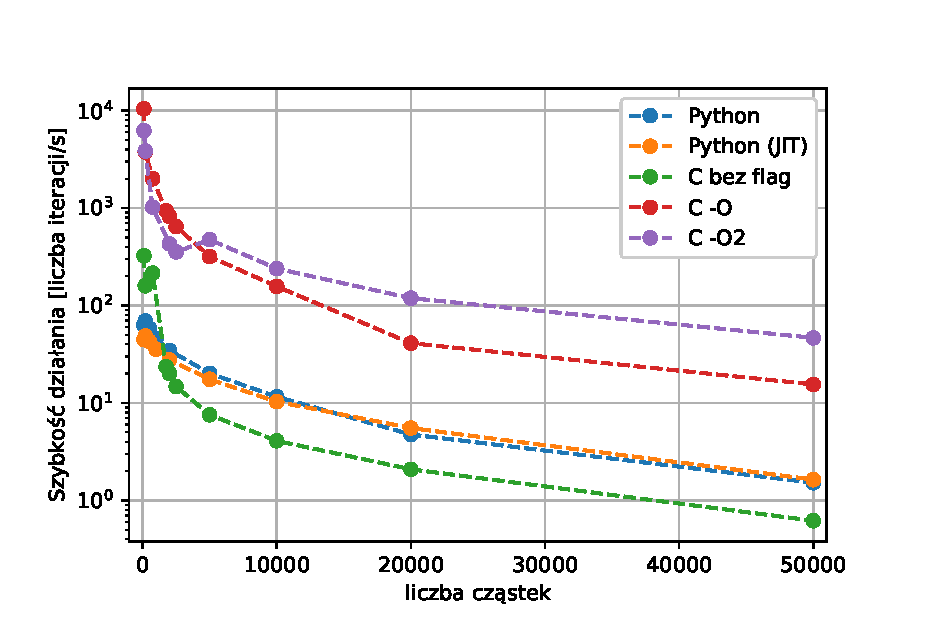
\includegraphics[width=\textwidth]{Images/speeds}
  \caption{Szybkość działania symulacji}\label{fig:runspeed}
\end{figure}
